\section{Definujte a vysvětlete základní pojmy (aktiva, hrozba, ochrana, bezpečnost, zranitelnost, riziko, incident a~dopad).}

\begin{table}[ht]
\begin{tabular}{l|l}
\textbf{aktiva}       & cokoliv cenného: data, služby, hardware, software, \dots \\
\textbf{hrozba}       & možnost ztráty aktiv \\
\textbf{ochrana}      & opatření ke~snížení rizika, četnosti nebo velikosti ztrát \\
\textbf{bezpečnost}   & stav, kdy riziko ztráty aktiv nepřesahuje určitou míru \\
\textbf{zranitelnost} & místo bez~dostatečné ochrany \\
\textbf{incident}     & realizace hrozby \\
\textbf{dopad}        & důsledek útoku, rozsah škod \\
\end{tabular}
\end{table}

\clearpage
\section{Bezpečná konfigurace přepínače a směrovače (základní postupy konfigurace, bezpečnostní funkce, útoky, Port Security, port Fast, hardening).}

L1:~rozbočovač (hub) a~opakovač (repeater), L2:~most (bridge) a~přepínač (switch), L3:~směrovač (router), přepínač (switch) a~brána (gateway), L4-L7:~sondy, brány, firewally, \dots

\subsection{Konfigurace}
\label{question2-1}

Jako v~případě veškerého síťového hardware je třeba \textbf{fyzicky zabezpečit přístup} k~přepínači (klíče, kódy, biometrie), připojit UPS, nepoužívané fyzické porty umístit do~\enquote{mrtvé} VLAN (aby~nebylo možné jen tak připojit nové zařízení). Je nutné zkontrolovat \textbf{požadavky na~síťový přístup} (HTTPS, dostatečné SSH klíče, logování přístupů a~manipulace, ACL), \textbf{vypnout služby a~porty} které nejsou využívány, \textbf{zapnout bezpečnostní funkce} (\href{https://en.wikipedia.org/wiki/DHCP_snooping}{DHCP Snooping}, \href{https://en.wikipedia.org/wiki/MAC_filtering}{MAC filtering/Port Security}, AAA, IPS, VPN). Také je třeba \textbf{zálohovat} konfigurace, nastavení testovat a~ověřovat, \textbf{aktualizovat} software i~firmware.

% TODO Tuto sekci je třeba projít a zkontrolovat, nevyznám se v tom dost na to, abych tomu plně věřil
\subsection{Zabezpečení přepínače}

\textbf{\href{https://en.wikipedia.org/wiki/MAC_filtering}{Port Security}} je omezení počtu MAC adres na~port/ochrana před~MAC útoky. \textbf{PortFast} nastavení porty na~forwarding state ihned po~zapojení (připojení stanic a~serverů). \textbf{BPDU Guard} chrání síť před~zasíláním BPDU zpráv (Spanning Tree) na~porty, které by takové zprávy v~normálním provozu z~těchto portů nedostaly. \textbf{Root Guard} zabraňuje nahrazení Root Bridge \emph{spoofovanou} zprávou od~útočníka, nastaví všechny root porty pro~STP.

Mezi útoky patří \textbf{MAC address spoofing} (příjem cizích dat pomocí nelegitimní změny směrovacích tabulek), \textbf{ARP Poisoning} (úprava ARP cache vede k~MitM), \textbf{Rough DHCP Server Spoofing} (falešný DHCP server odpovídá rychleji $\rightarrow$ MitM, DoS), \textbf{DHCP Starvation} (DHCP je zaplaven velkým množstvím dotazů s~cílem vyčerpání paměti IP adres), \textbf{STP Manipulation} (útočník jako Root Bridge pro~příjem provozu v~síti), \textbf{MAC address table overflow} (vyčerpá se MAC tabulka adres na~přepínači, který se přepne na~HUB a~data posílá všemi porty), \textbf{LAN storm} (přepínače přeposílají broadcast všemi porty, čímž se~přetíží CPU a~dojde k~DoS).

\subsection{Zabezpečení směrovače}

Bezpečná konfigurace je~popsána výše v~podkapitole \ref{question2-1}.

Mezi typické útoky na~směrovače patří pokusy o~\textbf{průnik do~nastavení} (zneužití výchozích hesel), \textbf{Routing Table Poisoning} (\emph{spoofování} routovacích protokolů a~vyvolání nežádoucích změn ve~směrovacích tabulkách), \textbf{Hit and Run} (posílání škodlivých paketů v~náhodných intervalech), \textbf{(D)DoS} (vytížení CPU/RAM velkým množstvím paketů, logické útoky typu \href{https://en.wikipedia.org/wiki/Christmas_tree_packet}{Christmas tree packet} attack).

\clearpage
\section{Problematika logování, hlavní cíle a rozdělení (definice logu, základní kategorie, formát, obsah logu, struktura záznamu, ochrana logů).}

\textbf{Log}, záznamová data, logovací zpráva je soubor nebo sada souborů obsahujících záznamy reprezentující popis konkrétní události, která nastala ve~sledovaném systému.

\subsection{Úrovně}

-- \textbf{ladící} (\texttt{DEBUG}): využívané při~vývoji a~hledání problémů, \\
-- \textbf{informační} (\texttt{INFO}): popisují stavy a~události, \\
-- \textbf{varovné} (\texttt{WARNING}): chybějící funkce nebo~součást systému, \\
-- \textbf{chybové} (\texttt{ERROR}): chyby ohrožující funkčnost systému, \\
-- \textbf{pohotovostní} (\texttt{CRITICAL}): událost spojená s~bezpečností nebo stav, ve~kterém sytém již dále nedokáže pracovat.

\subsection{Formát}

\textbf{Textový} formát má výhodu ve~skutečnosti, že ho lze otevřít v~jakémkoliv textovém editoru. Jeho vytváření je nenáročné na~systémové prostředky, existuje společná syntaxe pro~mnoho aplikací. \\
\textbf{Binární} formát lze číst pouze k~tomu určeným programem. Binární logy bývají menší než textové (data lze ukládat efektivnějí), lépe se ukládají do~databáze a~mají lepší optimalizaci využíti prostředků. Binární logování využívá například OS~Windows nebo Systemd.

\subsection{Obsah}

Každý záznam musí mít časové razítko, aby bylo v~případě problémů lehké zjistit posloupnost událostí. Také by měl obsahovat zdroj, který záleží na~typu logu: aplikační log by měl ukládat soubor či funkci, systémový program a~uživatele, síťový konkrétní stroj a~jeho adresu. Nesmí dojít k~ukládání hesel nebo klíčů.

Každému záznamu je také přiřazena úroveň pro~účely filtrace a~oddělení informačních údajů od~těch, kterým je potřeba věnovat zvýšenou pozornost. A~také musí být obsažena informace samotná, včetně informace o~chybě (\emph{traceback}), je-li k~dispozici.

\subsection{Ochrana a~manipulace}

Administrátor systému by měl mít přehled o~souborech, do~kterých logy zapisují klíčové programy a~démony (přihlašování, změna nastavení systému). Tyto logy by měly být zálohovány a~chráněny -- v~případě existence centrálního logovacího serveru je potřeba zajistit jejich bezpečnost i~při~přenosu po~síti.

\clearpage
\section{Definice operací nutných k~aplikaci automatické analýzy logů (blokové schéma včetně popisu funkce jednotlivých bloků). Jakým způsobem je realizován blok korelace při~detekci známých a~neznámých událostí.}

\begin{wrapfigure}{r}{0.35\textwidth}
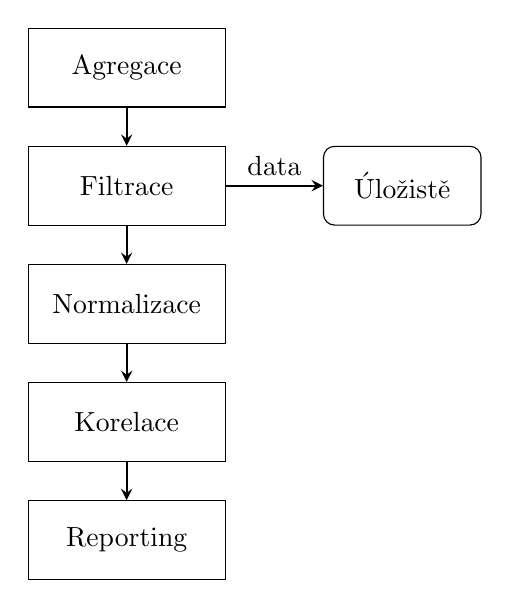
\begin{tikzpicture}[node distance=1.5cm]
\tikzstyle{block} = [rectangle, minimum width=2.5cm, minimum height=1cm, text centered, draw=black]
\tikzstyle{rounded} = [rectangle, rounded corners, minimum width=2cm, minimum height=1cm, text centered, draw=black]
\tikzstyle{arrow} = [thick,->,>=stealth]
%
\node (agregace)    [block] {Agregace};
\node (filtrace)    [block, below of=agregace] {Filtrace};
\node (úložiště)    [rounded, right of=filtrace, xshift=2cm] {Úložistě};
\node (normalizace) [block, below of=filtrace] {Normalizace};
\node (korelace)    [block, below of=normalizace] {Korelace};
\node (reporting)   [block, below of=korelace] {Reporting};
%
\draw [arrow] (agregace) -- (filtrace);
\draw [arrow] (filtrace) -- node[anchor=south] {data} (úložiště);
\draw [arrow] (filtrace) -- (normalizace);
\draw [arrow] (normalizace) -- (korelace);
\draw [arrow] (korelace) -- (reporting);
\end{tikzpicture}
\end{wrapfigure}

Při~\textbf{agregaci} začíná proces stahování záznamů na~jedno centrální místo. \textbf{Filtrace} je analýza surových dat a~rozhodování, která data jsou potřebná. \textbf{Normalizace} je úprava záznamů na~společný formát (který využívá databáze a~analytické systémy). \textbf{Korelace} je spojení podobných i~zcela odlišných událostí ve~znalost o~větší probíhající události. Představuje nejproblematičtější blok. Výsledná data jsou posílána e-mailem, zobrazena graficky odlišeným způsobem nebo jsou nějakou formou předložena lidskému operátorovi, který vykoná další akce.

V~případě incidentu, nebo i~při~pravidelné kontrole, lze využívat filtraci i~další programy, které hlídají zaznamenané události. Při~ruční analýze lze využít základní nástroje jako \texttt{tail}, \texttt{cat}, \texttt{grep} nebo Event Viewer.

\subsection{Detekce signatur (známých událostí)}

Shromažďovaná data jsou analyzována a~sledována. V~případě aktivace pravidla je realizována akce -- upozornění, obrana. Automatické SIEM (\emph{Security Information and~Event Management}) systémy nepokrývají všechny potřeby organizace a~velkou část korelací událostí je~nutné doprogramovat.

\subsection{Detekce anomálií (neznámých událostí)}

\textbf{Frekvenční model} počítá výskyty definovaného jevu za~pevně daný okamžik. \textbf{Referenční model} porovnáva model \enquote{normálního} chování a~sleduje, zda se sledované jevy pohybují v~povolených odchylkách -- data jsou sbírána a~porovnávána s~modelem. Přesnost je velmi závislá na~množství a~kvalitě dat ze~kterých byl model vytvořen. \textbf{Model strojového učení} klasifikuje vstupní data do~tříd a~shlukuje je do~skupin s~posobnými vlastnostmi.

Anomáliemi mohou být nadměrný provoz, změna chování síťového prvku, přihlášení pomocí VPN mimo pracovní hodiny, opakovaná neúspěšná přihlášení, přihlášení z~více IP během krátké doby, \dots

\begin{table}[ht]
\centering
\begin{tabular}{l|ccccc|l}
\textbf{klasifikovaná data} & NOP & NPP & FWA & VPNM & LF  & \textbf{odhadnutý výsledek} \\
\hline
brute force                 &     &     & ano &      & ano & --- \\
DDoS                        &     & ano & ano &      &     & --- \\
data loss                   & ano &     & ano & ano  &     & --- \\
\hline
--- & ano & & ano & & ano & brute force \\
--- & ano & & ano & ano & & data loss \\
\end{tabular}
\end{table}


\clearpage
\section{Detekce nepříznivých událostí na základě signatur a~anomálií, systémy IDS/IPS (vzájemný vztah, efektivita a ladění, umístění, základní architektura, zástupci, referenční model).}

\emph{Intrusion Detection Systems} odchytávají pakety a~provádí jejich analýzu, \emph{Intrusion Prevention Systems} k~tomu umí vytvářet vlastní aktivitu v~potlačování nevhodné aktivity.

Typicky jsou nasazeny \enquote{inline} jako síťové firewally. Umístění je rozhodující pro~jejich správnou funkčnost, často to bývá mezi komponetnami síťové infrastruktury.

\begin{figure}[ht]
\centering
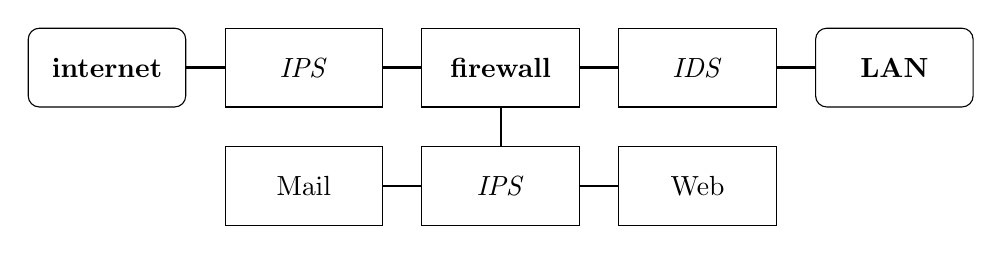
\begin{tikzpicture}[node distance=2.5cm]
\tikzstyle{block} = [rectangle, minimum width=2cm, minimum height=1cm, text centered, draw=black]
\tikzstyle{rounded} = [rectangle, rounded corners, minimum width=2cm, minimum height=1cm, text centered, draw=black]
\tikzstyle{arrow} = [thick,-,>=stealth]
%
\node (internet) [rounded] {\textbf{internet}};
\node (ids-out) [block, right of=internet] {\emph{IPS}};
\node (firewall) [block, right of=ids-out] {\textbf{firewall}};
\node (ids-server) [block, below of=firewall, yshift=1cm] {\emph{IPS}};
\node (server1) [block, left of=ids-server] {Mail};
\node (server2) [block, right of=ids-server] {Web};
\node (ids-in) [block, right of=firewall] {\emph{IDS}};
\node (lan) [rounded, right of=ids-in] {\textbf{LAN}};
%
\draw [arrow] (internet) -- (ids-out);
\draw [arrow] (ids-out) -- (firewall);
\draw [arrow] (firewall) -- (ids-server);
\draw [arrow] (ids-server) -- (server1);
\draw [arrow] (ids-server) -- (server2);
\draw [arrow] (firewall) -- (ids-in);
\draw [arrow] (ids-in) -- (lan);
\end{tikzpicture}
\end{figure}

IDS/IPS existují ve~třech variantách: \textbf{komplexní} zařízení je hardware a~software vytvořený k~efektivnímu odchytávání a~analýze provozu, \textbf{softwarová} zařízení jsou speciální programy nainstalované na~server (Snort, Suricata), \textbf{cloudová} jsou dostupná od~ISP (Radware, F5).

V~\textbf{jednovrstvé} architektuře je IPS/IDS tvořen jedinou komponentou, která obstarává všechny funkce. Ve~\textbf{vícevrstvé} architektuře (zpravidla třívrstvé) existuje jeden manažer (analyzuje hlášení a~realizuje opatření), kterému náleží agenti (analyzují protokoly a~služby), kteří využívají senzory (monitorující provoz a~předávající data).

\subsection{Referenční model IPS}

\begin{figure}[ht]
\centering
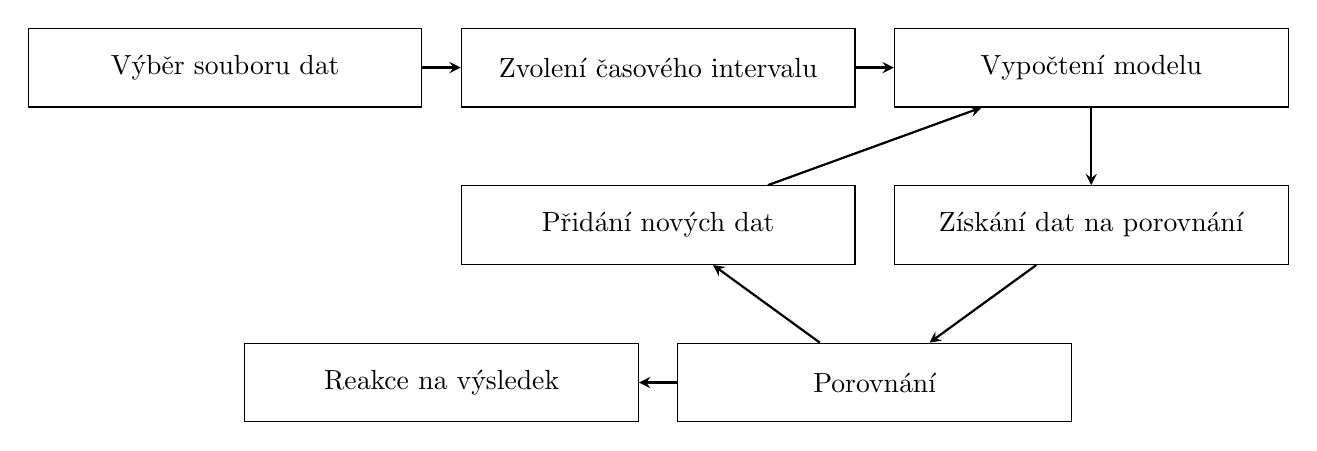
\begin{tikzpicture}[node distance=5.5cm]
\tikzstyle{block} = [rectangle, minimum width=5cm, minimum height=1cm, text centered, draw=black]
\tikzstyle{arrow} = [thick,->,>=stealth]
%
\node (1) [block] {Výběr souboru dat};
\node (2) [block, right of=1]                              {Zvolení časového intervalu};
\node (3) [block, right of=2]                              {Vypočtení modelu};
\node (4) [block, below of=3, yshift=3.5cm]                {Získání dat na~porovnání};
\node (5) [block, below of=2, yshift=1.5cm, xshift=2.75cm] {Porovnání};
\node (6) [block, below of=2, yshift=3.5cm]                {Přidání nových dat};
\node (7) [block, left of=5]                               {Reakce na~výsledek};
%
\draw [arrow] (1) -- (2);
\draw [arrow] (2) -- (3);
\draw [arrow] (3) -- (4);
\draw [arrow] (4) -- (5);
\draw [arrow] (5) -- (6);
\draw [arrow] (6) -- (3);
\draw [arrow] (5) -- (7);
\end{tikzpicture}
\end{figure}

\clearpage

\section{Dělení penetračních testů (dle znalosti, způsobu realizace a cíle), metodologie testování (pět kroků testování). Penetrační testování webových aplikací (OWASP, průzkum prostředí, závěrečný report).}

Penetrační testování je posouzení bezpečnosti pomocí pokusu o~průnik do~testovaného systému. Umožňuje komplexní prozkoušení nově nasazených aplikací, bezpečnostních systémů, firewallů, IPS/IDS apod. Nutností je mít souhlas majitele systému.\footnote{\textit{Pozor!} Posouzení zranitelnosti není to stejné jako penetrační test. \textit{Penetrační test} je komplexní činností, kde se hledají, identifikují a~následně zneužívají (v~omezeném rozsahu) zranitelnosti. Oproti tomu \textit{posouzení zranitelností} je především automatizovanou činností, která zranitelnosti hledá, ale nedemonstruje jejich zneužití.}

\subsection{Dělení penetračních testů}

\subsubsection*{Dle znalosti:}

\begin{itemize}
    \item \textbf{Black Box}: tester zná jen vstupy a~potenciální výstupy systému, neví nic o~vnitřním uspořádání, tj. je v~pozici běžného uživatele. U~tohoto typu testování se vyžaduje především dobrá znalost skenovacích technik a~mapování sítě/systému. \textit{Nevýhodou} může být, že pokud nedojde k proniknutí do sítě, nebude otestována interní bezpečnost.  
    
    \item \textbf{White Box}: k~dispozici má topologii sítě, přístupové údaje, dokumentaci, tj. je v~pozici vývojáře/technika. Dopadem tohoto velkého množství informací je fakt, že testeři stráví hodně času studií a~pochopením systému, oproti samotnému testování. Často se využívají techniky jak statické, tak dynamické analýzy kódu. \textit{Nevýhodou} může být, že testeři nepřemýšlejí jako skutečný útočník.
    
    \item \textbf{Grey Box}: kombinace dvou předchozích, k~dispozici jsou pouze základní znalosti o~systému. \textit{Výhodou} je, že testeři se mohou soustředit na testování zranitelné části systému, namísto prohledávání systému od nuly. 
\end{itemize}
 
\subsubsection*{Dle realizace:}

\begin{itemize}
    \item \textbf{Automatizované testy} využívají specializovaných nástrojů schopných detekce vlastností a~chyb zkoumaného systému. Výhodou je rychlost či~velké pokrytí \emph{attack surface}, tester však musí znát limitace aplikace a~možnosti jejího nastavení.
    
    \item \textbf{Manuální testy} se provádí ručně a~jsou tedy časově mnohem náročnější a~od~testera vyžadují hlubokou znalost oblasti, umožní však testování na~míru a~pokrytí detailů, které automatizované testy nepokryjí. Tyto dvě formy se v~praxi kombinují.
\end{itemize}
\subsubsection*{Dle cíle:}

Síťová infrastruktura. Webové aplikace. Programy. Telefonní aplikace. IoT zařízení. Fyzický pentest.\footnote{Penetrační testy lze dále rozdělit na externí a interní. Záleží na počáteční pozici testera, tj. mimo/uvnitř sítě.} 

\subsection{Metodologie}

\begin{table}[h]
\centering
\begin{tabular}{p{3cm}|p{12cm}}
plánování      & určují se~detailní cíle a~časový plán, vymezují se priority \\
sběr informací & zjištění informací o~síti/systému: IP rozsahy, porty, služby \\
odhalování     & zjištění typu a~verzí služeb běžících za~otevřenými porty \\
zneužití       & využívání nalezených zranitelností \\
report         & předání výsledků, které povedou ke~zvýšení bezpečnosti \\
\end{tabular}
\end{table}

\subsection{Testování webových aplikací}

\textbf{OWASP} (Open Web Application Security Project) je nezisková organizace zaměřená na~zlepšování bezpečnosti software. Jejím cílem je neomezený přístup jednotlivců i~organizací k~informacím o~bezpečnostních hrozbách. Mezi jejich neznámější publikace patří: OWASP top 10, ASVS (Application Security Verification Standard), OWASP Web Security Testing Guide

\subsubsection{OWASP Top 10}

Publikace shrnující aktuálních deset nejhorších zranitelností. Vychází z~domluvy firem z~odvětví a~OWASP, nemusí tedy nutně znamenat, že se vyskytují nejčastěji. Postupně se jedná o zranitelnosti (2017):

\begin{enumerate}[noitemsep]
    \item Injekce (SQL injection, Code injection)
    \item Nekorektní funkce autentizace (obecné chyby autentizačních mechanismů)
    \item Odhalení citlivých dat (např. nezabezpečená komunikace aplikace jako HTTP/FTP, výpis chyb na~stránce, \dots)
    \item XML externí entity tj. XXE (code execution přes~chybu v~parseru XML\footnote{XXE: \url{https://www.youtube.com/watch?v=gjm6VHZa_8s}.})
    \item Chybná kontrola přístupu (chyba v~ACL)
    \item Špatná konfigurace bezpečnostních politik (nenastavení lockout mechanismu po~určitém počtu neúspěšných přihlášení)
    \item Cross Site Scripting tj. XSS (vykonávání JavaScriptu na~straně uživatele\footnote{XSS: \url{https://www.youtube.com/watch?v=EoaDgUgS6QA}.})
    \item Nebezpečná deserializace (při~převodu binárních dat na~interní reprezentaci v~programu může dojít k~vykonání kódu\footnote{Deserializace: \url{https://www.youtube.com/watch?v=HaW15aMzBUM}.})
    \item Užívání komponent se známou zranitelností
    \item Nedostatek loggingu a~monitoringu
\end{enumerate}

\clearpage

\subsubsection{OWASP Testing Guide}

Rozděluje penetrační test na dvě fáze: \textbf{Pasivní fáze} a \textbf{Aktivní fáze}.
\\

V pasivní fázi dochází k tzv. \textit{fingerprintingu} (tj. k průzkumu prostředí). Na konci této fáze by útočník měl mít základní znalosti o prostředí webu, jako přístupové body, funkcionality a obsah. Jedna ze základních metod je využití veřejně dostupných informací z vyhledávačů jako Google, DuckDuckGo apod. (tzv. Google Dorking) Dále lze využívat HTTP proxy (jako BurpSuite) pro prozkoumání zaslaných HTTP žádostí za účelem identifikace OS serveru nebo typu serveru (Apache, Microsoft, Apache Tomcat, ...). 
\\

V aktivní fázi už dochází k interpetaci dat získaných z fingerprintingu a pokusy o exploitaci. Všechny zranitelnosti, payloady a~nevydařené útoky by měly být řádně zapsány. To umožní později sepsat koherentní a~komplexní report. 

\subsubsection{Report}

V \textbf{OWASP Web Security Testing Guide} je uvedeno že dobrý report je základ penetračního testu. Bez něj nelze prezentovat výsledky a zajistit, že chyby budou opraveny. Rozděluje report na čtyři části:

\begin{table}[ht]
\centering
\begin{tabular}{p{1.5cm}|p{13.5cm}}
Úvod      &  prostor pro obsah, jména členů týmu, limity testování, časové rozmezí testu\\
Shrnutí   &  cíl testu, shrnutí dopadů z ekonomického a compliance hlediska, návrhy pro~budoucí zlepšení \\
Nálezy    &  výpis všech nalezených zranitelností, všechny zranitelnosti by měly obsahovat co nejvíce detailní informace \\
Dodatky   & použité metody, nástroje, vysvětlení závažnosti, relevantní výstupy nástrojů, \dots \\
\end{tabular}
\end{table}

Více např. \url{https://owasp.org/www-project-web-security-testing-guide/v42/5-Reporting/README.html}.


\clearpage
\section{(D)DoS útoky (princip, rozdělení, popis základních útoků: SYN Flood, HTTP Flood, DNS reflection, Ping of Death, Slow-Loris). Zátěžové testování (typy testů, nejznámější nástroje).}

\textbf{DDoS} (\emph{Distributed Denial of~Services}) je DoS útok realizovaný z~více uzlů, které s~hlavním útočníkem spolupracují a~napadají cílový uzel. \\
\textbf{Botnet} je skupina uzlů (až statisíce), které zpravidla bez~vědomí svých majitelů útočí na~cíle na~internetu. Svému majiteli vytváří zpravidla zisk nebo jiné prostředky (exploit, trojan, pronájem, těžba kryptoměn, krádež dat).

% TODO Možná by se hodilo ty útoky nalinkovat, pokud k nim něco existuje?
\subsection{Typy útoků}

\subsubsection{Záplavové útoky}

\textbf{ARP flood}: ARP dotazy \\
\textbf{RST flood}: pakety obsahují falešné IP adresy s~parametrem RST, který resetuje spojení \\
\textbf{SYN flood}: otevření spojení bez~následného potvrzení\footnote{\url{https://www.cloudflare.com/learning/ddos/syn-flood-ddos-attack/}} \\
\textbf{HTTP flood}: legitimní, ale náročné GET a~POST dotazy \\
\textbf{UDP flood}: legitimní UDP datagramy \\
\textbf{PingSweep}: zprávy od~uzlů požadují odpovědi od~cílového systému\footnote{\url{https://www.netscout.com/what-is-ddos/icmp-flood}} \\
\textbf{Smurf}: ICMP pakety se \emph{spoofovanou} adresou oběti jsou posílány na~broadcast adresu \\
\textbf{Reflection attack}: malý dotaz se~zdrojovou adresou oběti: DNS/NTP amplifikace\footnote{\url{https://www.cloudflare.com/learning/ddos/dns-amplification-ddos-attack/}}
 

\subsubsection{Logické útoky}

\textbf{Teardrop}: fragmenty paketů se špatně nastaveným offsetem: cíl není schopen správně sestavit celý packet \\
\textbf{Land}: TCP-SYN mají cílovou IP adresu i~port shodné se~zdrojovou adresou \\
\textbf{Ping of~Death}: ICMP ping s~velikostí nad~65kB \\
\textbf{ReDoS}: extrémní zátěž pomocí regulérních výrazů \\
\href{https://www.youtube.com/watch?v=XiFkyR35v2Y}{\textbf{XMasTree}}: TCP paket má v~hlavičce nastaveny příznaky FIN, URG, PST \\
\textbf{Slow-Loris}: nekompletní pomalý GET dotaz

\clearpage

\subsection{Detekce a~mitigace}

Detekce signatur a~anomálií. Robustní a~bezpečná síťová infrastruktura; firewally, IDS, honeypoty, redundantní linky a~servery; vysokorychlostní DDoS filtry; blacklisting \& whitelisting; \emph{tarpit} (udržení příchozích spojení v~open-state, snížení TCP window na~nulu); rate limiting na~směrovačích; filtrace na~základě reputace zdroje (IP rozsah, geolokace, služba).

\subsection{Zátěžové testování}

Lze testovat sítě jako celek, síťová zařízení (servery, routery, firewally), koncové stanice (počítače, telefony) nebo aplikační vrstvu (webové služby, operační systémy, aplikace).

Postup testování: \textbf{definice} (specifikace cíle, požadavků a~běžného provozu), \textbf{příprava} (nastavení sítě a~testeru), \textbf{realizace} (monitoring, opakování), \textbf{vyhodnocení} (dokumentace).

Hlídanými \textbf{parametry} jsou: doba, počet dotazů, čas na~dotaz, dotazy za~čas, přenesená data, distribuční rozložení odpovědí, \dots

\textbf{Performance test} je zatížení systému definovanou zátěží pro~změření chování. \textbf{Stress test} je postupné zatěžování narůstajícím počtem paralelních spojení. \textbf{Soak test} je dlouhodobé testování. \textbf{Failover test} je ověření chování systému v~případě selhání. \textbf{Targeted infrastructure test} slouží k~detekci nejslabších míst. \textbf{Volume test} je ověření chování při~zvýšeném objemu dat.

Je vhodné testovat mimo běžnou špičku, aby nebyla ohrožena finanční (služby zákazníkům) nebo bezpečnostná strana sítě.

\subsection{Software testery}

Avalanche (hardware, do~40Gbps), Apache jMeter, LOIC.

\clearpage
\section{Netechnické typy útoků (sociální inženýrství, phising; používané techniky), útoky MitM (ARP spoofing, DNS spoofing, SSL strip, SSL sniff).}

\textbf{sociální inženýrství}: psychická manipulace s~lidmi za~účelem zisku informací, přístupu ke~službě nebo provedení podvodu \\
\textbf{phishing}: kontaktování uživatelů s~cílem získání citlivých informaci pro~škodlivé účely \\
\textbf{spear phishing}: phishing mířený na~konkrétní osoby \\
\textbf{clone phishing}: vytvoření phishing zprávy z~původně legitimní \\
\textbf{whaling}: cílení na~vlivné představitele firm či organizací nebo na~veřejné osoby \\
\textbf{baiting}: zanechání malware na~médiu, které má oběť objevit a~připojit ke~svému sytému \\
vydávání se za~jinou profesi (technická podpora, údržba) \\
\textbf{tailgating}: průnik do~chráněných prostor s~nevědomou pomocí legitimního uživatele \\
\textbf{insider threats}: hrozby od~vnitřního uživatele

\subsection*{Phishing}

\textbf{Vektory} bývají e-mail, sociální sítě, webové portály nebo instant messaging. \textbf{Cílem} bývá přístup k~bankovnictví, webovým portálům, sociálním sítím nebo IT službám. \textbf{Obranou} je legislativa, školení uživatelů, veřejná informovanost, technická opatření (e-mail filtering, vynucení 2FA).

Využívá se \textbf{manipulace s~odkazy} (modifikace URL, rozdíl mezi obsahem a~cílem \texttt{<a>} tagu pomocí JS), \textbf{obcházení filtrace} (využití obrázků či videa místo textu), \textbf{website tampering} (podvržení webových stránek) nebo \textbf{covert redirect} (přesměrování odkazů na~phishing stránky s~XSS/falešným přihlášením).

\subsection{MitM}

\subsubsection{ARP spoofing}

Také \emph{ARP cache Poisoning} nebo \emph{ARP poison Routing}. Jde o~způsob podvrhnutí ARP zpráv na~lokální síti; cílem je asociovat útočníkovu MAC adresu s~IP adresou jiného síťového prvku (brána) a~routovat veškerou komunikaci místo něj. Útočník může způsobit DoS (zahazováním některých paketů) nebo MitM (úpravou dat).

\begin{figure}[ht]
\centering
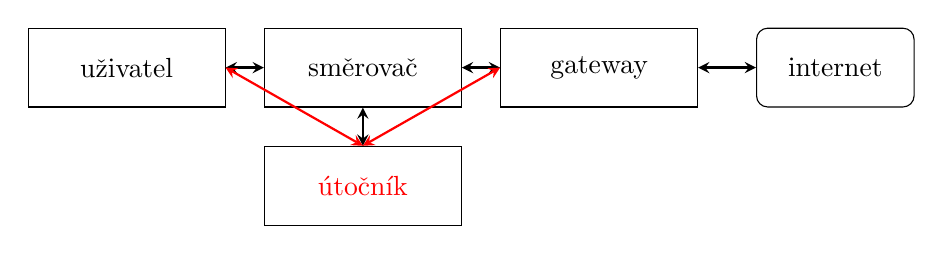
\begin{tikzpicture}[node distance=3cm]
\tikzstyle{block} = [rectangle, minimum width=2.5cm, minimum height=1cm, text centered, draw=black]
\tikzstyle{rounded} = [rectangle, rounded corners, minimum width=2cm, minimum height=1cm, text centered, draw=black]
\tikzstyle{arrow} = [thick,<->,>=stealth]
%
\node (user)     [block]                                  {uživatel};
\node (switch)   [block,   right of=user]                 {směrovač};
\node (gateway)  [block,   right of=switch]               {gateway};
\node (internet) [rounded, right of=gateway]              {internet};
\node (attacker) [block,   below of=switch, yshift=1.5cm] {\color{red} útočník};
%
\draw [arrow]      (user)           -- (switch);
\draw [arrow]      (switch)         -- (gateway);
\draw [arrow]      (gateway)        -- (internet);
\draw [arrow]      (switch)         -- (attacker);
\draw [arrow, red] (user.east)      -- (attacker.north);
\draw [arrow, red] (attacker.north) -- (gateway.west);
\end{tikzpicture}
\caption*{Síť pod~ARP spoof útokem}
\end{figure}

Při~překladu lokální IP adresy na~MAC dochází k~zaslání broadcast paketu, na~který zařízení s~požadovanou IP adresou pošle odpověď. Tyto zprávy nejsou nijak autentizované, ARP je stateless protokol a~všechna zařízení na~síti automaticky \emph{cachují} ARP odpovědi bez~ohledu na to, jestli o~ně požádaly.

Ochranou může být integrace s~DHCP serverem nebo monitoring ARP provozu.

\subsubsection{DNS spoofing}

Způsob podvrhnutí DNS zpráv a~otrávení DNS cache s~účelem směrovat některé DNS záznamy na~falešné IP adresy. V~normálním prostředí plní roli neautoritativního DNS serveru lokální směrovač, který směrovací data získává od~dalšího DNS serveru (síť, ISP, autoritativní DNS server).

DNSSEC zaručuje bezpečnost komunikace s~DNS servery. Všechny odpovědi z~DNSSEC zón jsou podepsány. Krom \texttt{A}/\texttt{AAAA} záznamů lze chránit i~\texttt{TXT}, \texttt{MX} a~další: SSHFP (SSH klíče vázané na~hostname) nebo IPSec klíče. Zajišťuje pouze autentizaci, ne důvěrnost.

\subsubsection{SSL strip}

Degradace HTTPS spojení na~HTTP. Tři roky po~jeho \enquote{objevení} v~roce 2009 bylo vydáno \href{https://datatracker.ietf.org/doc/html/rfc6797}{RFC~6797: HTTP Strict Transport Security (HSTS)}, zavádějící HTTP hlavičku \texttt{Strict-Transport-Security}. Klienti podporující HSTS musí upgradovat na~HTTPS \emph{před}~připojením k~webu, a~pokud není možné TLS spojení navázat (nedůvěryhodný certifikát), spojení by mělo být ukončeno a~na~web by neměl být povolen přístup.%
\footnote{Mezi limitace HSTS patří náchylnost na~NTP manipulaci (platnost HSTS hlavičky je určena časem: \texttt{Strict-Transport-Security: max-age=31536000}) nebo~na~stripping při~první návštěvě, protože se HSTS hlavička přenáší až~první odpovědí serveru.}

\subsubsection{SSL sniff}

Zachycení TLS. Útočník musí mít k~dispozici certifikát kterému důvěřuje prohlížeč, tj.~ukradený certifikát podepsaný CA, nebo falešný a~importovaný do~prohlížeče/systému oběti.

\clearpage
\section{Protokoly IPsec a TLS (princip, umístění TCP/IP, průběh komunikace, autentizace, utajení a integrita dat).}

\subsection{IPSec}

Pracuje na~síťové vrstvě (L3): end-to-end šifrování TCP/UDP komunikace mezi zařízeními s~IP adresou. Šifrují se~data v~paketech (transport) nebo pakety celé (tunnel), včetně podpory autentizace.

\begin{figure}[ht]
\centering
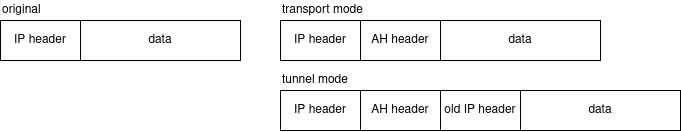
\includegraphics[width=\textwidth]{images/ipsec}
\end{figure}

\textbf{Authentication header} zajišťuje integritu a~autentičnost IP paketů, chrání proti replay útokům. \textbf{Encapsulationg Security Payloads} zajišťuje důvěrnost pomocí šifrování. \textbf{Security Association} popisuje IPSec spojení včetně parametrů zabezpečení. Aktivní spojení je uloženo v~databázi (SAD), management a~pravidla jsou uložena v~SPD (\emph{Security Policy Database}).

Pro~ustanovení klíče IPSec využívá symetrickou kryptografii: pre-shared key, IKE1/2, Kerberos.

\begin{figure}[ht]
\centering
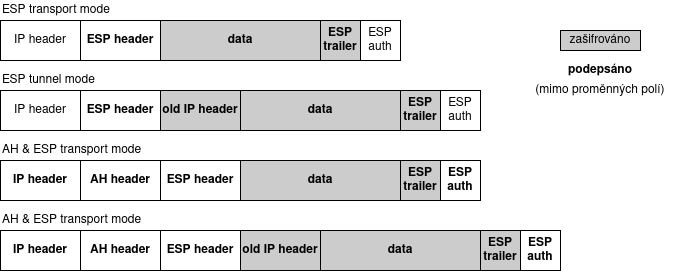
\includegraphics[width=\textwidth]{images/ipsec-modes}
\end{figure}

\clearpage
\subsection{TLS}

Pracuje na~transportní vrstvě (L4): end-to-end šifrování TCP/UDP mezi~klientem a~serverem, pro~aplikační vrstvu transparentní. Je~složen z~\textbf{handshake} (inicializace spoje, autentikace stran, ustanovení klíče), \textbf{record} (datový přenos, MAC autentizace) a~\textbf{alert} (notifikace chyb a~varování) protokolů.

Security strings, např.~\texttt{TLS\_ECDHE\_RSA\_WITH\_AES\_128\_GCM\_SHA256}.

\begin{itemize}[noitemsep]
\item Ustanovení klíče: ECDHE, DHE
\item Podpis: RSA, DSA, ECDSA
\item Šifrování: AEC-GCM, ChaCha
\item Hashování: SHA-256, SHA-384
\end{itemize}

\begin{figure}[ht]
\centering

\includegraphics[width=0.7\textwidth]{images/tls}
\caption*{Výměna zpráv v~TLS 1.2 a~TLS 1.3}
\end{figure}

\clearpage
% TODO WPA handshake není kompletní. Není popsáno co je GTK a jaké jsou obecně požadavky. Celá otázka by chtěla zrevidovat a doplnit
\section{Zabezpečení 802.11 (WPA2, používaná kryptografická primitiva, klíčové hospodářství, popis 4Way handshake, testování bezpečnosti).}

\textbf{WEP} (Wired Equivalent Privacy): nevhodná implementace šifrování, chybí management klíčů, předvídatelný obsah. Šifrování pomocí 64b/128b RC4 klíčů, integrita CRC-32, jednostranná autentizace. 2w~handshake: open system (pouze požadavek s~SSID sítě), 4w~handshake: požadavek s~SSID, nádhodný řetězec $r$, odpověď $E_{k_\mathrm{priv}}(r)$, přijmutí/odmítnutí. \\
\textbf{WPA} (WiFi Protected Access): rychlé vydání kvůli nedostatečné bezpečnostni WEP. Autentizace pomocí PSK/IEEE 802.1x, důvěrnost TKIP (Temporal Key Integrity Protocol) s~per-packet obměnou klíče, integrita MIC (Message Integrity Check). Zachována zpětná kompatibilita s~WEP. \\
\textbf{WPA2} (WPA II): Důvěrnost pomocí AES, integrita CCMP%
\footnote{Útok \href{https://krackattacks.com}{\textbf{KRACK}}: Key Reinstallation Attacks z~roku 2017.}%
. \\
\textbf{WPA3} (WPA III): AES-256-GCM, HMAC SHA-384. SAE (Simultaneous Authentication of~Equals) zajišťuje bezpečnější výměnu a~dopřednou bezpečnost v~Personal módu%
\footnote{V~dubnu 2019 byla ve~WPA3 objevena zranitelnost \href{https://wpa3.mathyvanhoef.com/}{\textbf{Dragonblood}} umožňující \emph{downgrade} spojení a~útok postranními kanály: umožnění zjištění hesla silou a~DoS útoku na~stanici.}%
.

\vspace*{1em}\noindent
\textbf{PMK} (Pairwise Master Key) je získán z~úspěšné autentizace (u~Enterprise zaslán serverem, u~Personal je shodný s~PSK, který se~odvozuje z~hesla%
\footnote{$\mathrm{PSK} = \mathrm{PBKDF2}(password, SSID, SSID\_length, \mathrm{rounds}=4096, \mathrm{output}=256)$, viz \href{https://datatracker.ietf.org/doc/html/rfc8018}{RFC~8018}.}%
), další klíče jsou z~něj derivovány hashováním: \\
\textbf{KCK} (Key Confirmation Key): autentizační zprávy MIC během čtyřcestné výměny, \\
\textbf{KEK} (Key Encryption Key): zajištění důvěrnostni dat během čtyřcestné výměny, \\
\textbf{TEK} (Temporary Encryption Key): šifrování dat v~TKIP a~CCMP, \\
\textbf{TMK} (Temporary MIC Key): autentizace dat v~TKIP.

\begin{table}[ht]
\centering
\begin{tabular}{ccc}
\textbf{klient} && \textbf{AP} \\
\hline
$\leftarrow$ & ANonce & $\leftarrow$ \\
vytvoření PTK && \\
$\rightarrow$ & SNonce + MIC & $\rightarrow$ \\
&& vytvoření PTK \\
$\leftarrow$ & GTK + MIC & $\leftarrow$ \\
$\rightarrow$ & ACK & $\rightarrow$ \\
\end{tabular}
\caption*{Čtyřcestná WPA výměna}
\end{table}

\begin{table}[ht]
\centering
\begin{tabular}{l|ccccc}
& \textbf{WPA-PSK} & \textbf{WPA} & \textbf{WPA2-PSK} & \textbf{WPA2} \\
\hline
\textbf{Autentizace} & PSK & 802.1x (PEAP) & PSK & 802.1x (PEAP) \\
\textbf{Šifrování} & TKIP (RC4) & TKIP (RC4) & CCMP (AES) & CCMP (AES) \\
\textbf{Enterprise} & nevhodné & dobrá úroveň & nevhodné & nejlepší úroveň \\
\textbf{Personal} & dobrá úroveň & nevhodné & nejlepší úroveň & nevhodné \\
\end{tabular}
\end{table}

\subsection{Testování bezpečnosti}

\textbf{WEP}: pasivní: \texttt{airodump-ng}, aktivní: \texttt{aireplay-ng} (Chopchop attack, Caffe Latte attack, \dots) \\
\textbf{WPA}: bruteforce (\texttt{airodump-ng}, \texttt{aircrack-ng}) \& dictionary/rainbow attacks \\
zmatení uživatele: vytvoření falešného AP a~vyzrazení hesla \\
automatické nástroje \texttt{wifite}, \texttt{fluxion}
